\documentclass[12pt, a4paper]{article}

% Acentuação
\RequirePackage[T1]{fontenc}
\RequirePackage[utf8]{inputenc}

% Configurando as margens
\usepackage[top = 2cm, bottom = 2cm, left = 3cm, right = 3cm]{geometry}
% Indentação do parágrafo
\setlength{\parindent}{2cm}
% Espaçamento entre parágrafo e texto
\setlength{\parskip}{1em}
% Espaçamento entre linhas
\renewcommand{\baselinestretch}{1.5}
% Identar o primeiro parágrafo das seções
\usepackage{indentfirst}
% Para usar símbolos como >=
\usepackage{amssymb}
% Para colocar texto entre $$ com \text{oi}
\usepackage{amsmath}
% Para usar listas com estilos específicos
\usepackage{enumerate}
% Para utilizar imagens
\usepackage{graphicx}

\renewcommand{\figurename}{Figura}

\begin{document}

	\input{Título.tex}

	\section{Introdução à pilares}
	Em estruturas de edifícios, os pilares são elementos verticais que tem a função primária de transmitir as \textbf{ações verticais} gravitacionais e de serviço e as \textbf{orizontais (vento)} às fundações, além de conferirem \textbf{estabilidade global} ao edifício. Os pilares usuais dos edifícios apresentam um comportamento de flexo-compressão, sendo as forças normais preponderantes.
Em edifícios de concreto armado, as seções dos pilares são geralmente \textbf{retangulares}.

% inserir imagem

Pilares de seção \textbf{quadrada} ou \textbf{circular} também podem ser considerados em projetos estruturais de edifícios.
Em virtude do tipo de material (concreto) e da solicitação preponderantemente de força de compressão, os pilares apresentam \textbf{rupturas frágeis}. A \textbf{ruína} de uma seção transversal de \textbf{um único pilar} pode ocasionar o \textbf{colapso} progressivo dos demais pavimentos.

As \textbf{disposições} dos pilares na planta de forma de um edifício são importantes, pois, junto com as vigas, formam \textbf{pórticos} que proporcionam \textbf{rigidez} e \textbf{estabilidade global} ao edifício.

Os pilares são peças estruturais que precisam ser projetadas \textbf{cuidadosamente} em termos de resistência, estabilidade e durabilidade, sempre respeitando as diretrizes e recomendações das \textbf{normas técnicas}.

O dimensionamento dos pilares é feito em função dos esforços externos solicitantes de cálculo, que compreendem as forças normais $(N_d)$ e os momentos fletores $(M_{dx}$ e $M_{dy})$.

	\section{Agressividade do ambiente}
	Está relacionada às \textbf{ações físicas} e \textbf{químicas} que atuam sobre as estruturas de concreto, independentemente das \textbf{ações mecânicas}, das variações térmicas, da retração e outras previstas no dimensionamento das estruturas.

Nos projetos das estruturas, a agressividade ambiental deve ser classificada de acordo com a Tabela 6.1 da ABNT NBR 6118 e pode ser avaliada segundo as condições de exposição da estrutura ou de suas partes. Conhecendo o ambiente em que a estrutura será construída, o projetista estrutural pode considerar uma condição de agressividade maior que a tabela.

% inserir tabela

Conforme a NBR 6118 - item 7.4: A durabilidade das estruturas é \textbf{altamente dependente} das características do concreto e da \textbf{espessura} e \textbf{qualidade} do concreto de cobrimento da armadura.

\textbf{Ensaios comprobatórios} de desempenho da durabilidade da estrutura frente ao tipo e classe de agressividade prevista em projeto devem estabelecer os parâmetros mínimos a serem atendidos. Na falta destes e devido à existência de uma \textbf{forte correspondência} entre a \textbf{relação água/cimento} e a \textbf{resistência do concreto} e sua \textbf{durabilidade}, permite-se que sejam adotados os requisitos mínimos da tabela abaixo:

\begin{table}[H]
\centering
\caption{Tabela 7.1 da NBR 6118.}
\begin{tabular}{|c|c|c|c|c|}
\hline
\multirow{2}{*}{Concreto} & \multicolumn{4}{c|}{Classe de Agressividade Ambiental (CAA)}                      \\ \cline{2-5} 
                          		& I                  & II                 & III                & IV                 \\ \hline
Relação a/c               & $\leqslant$ 0,65   & $\leqslant$ 0,6    & $\leqslant$ 0,55   & $\leqslant$ 0,45   \\ \hline
Classe de concreto        & $\geqslant$ C20 & $\geqslant$ C25 & $\geqslant$ C30 & $\geqslant$ C40 \\ \hline
\end{tabular}
\end{table}

	\section{Solicitações normais}
	Os pilares podem estar submetidos à forças normais e momentos fletores, gerando compressão simples e flexão composta.

\begin{itemize}

	\item \textbf{Compressão simples}: Também chamada de compressão centrada ou compresão uniforme, é caracterizada pela aplicação da força normal $(N_d)$ no centro geométrico da seção transversal do pilar.

		\begin{figure}[H]
			\begin{center}
				\caption{Solicitação normal acontecendo no centro geométrico da seção transversal do pilar.}    	
				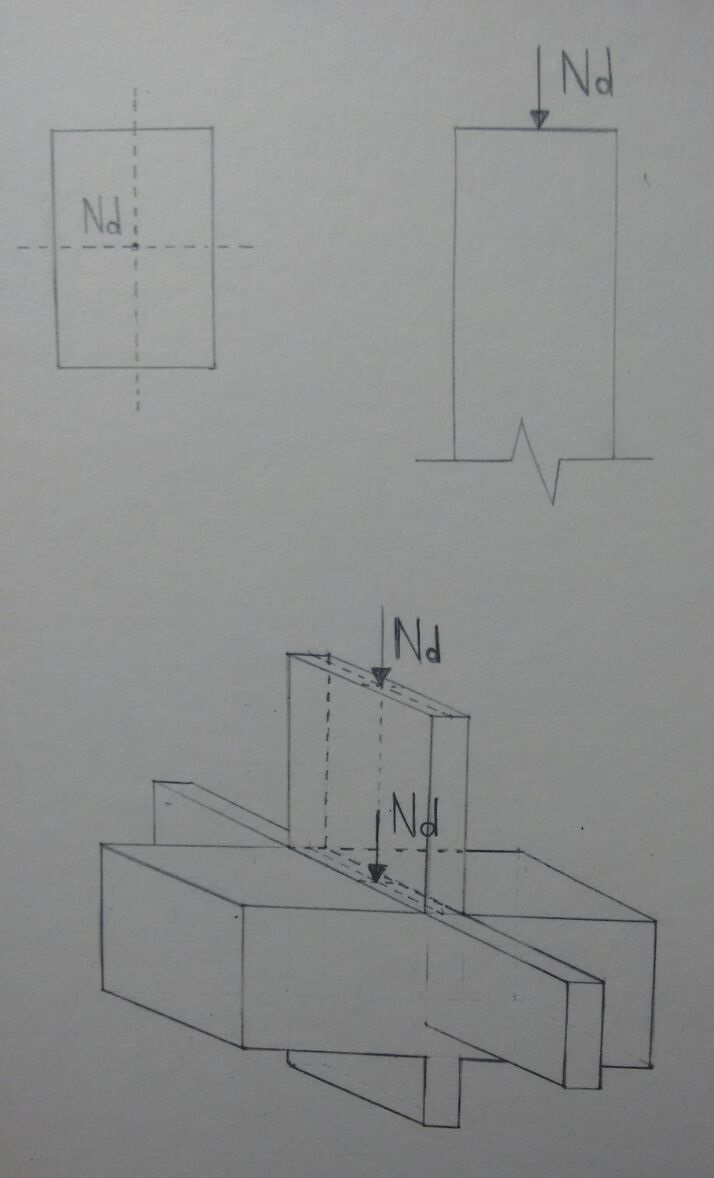
\includegraphics[height=0.5\textwidth]{Solicitacoes-normais/Imagens/Compressao-simples.jpg}
			\end{center}
		\end{figure}

	\item \textbf{Flexão composta}: Ocorre força normal e momento fletor sobre o pilar. Há dois casos:

		\begin{itemize}
     			\item \textit{Flexão composta normal (ou reta)}: Existe a força normal e um momento fletor em uma direção, sendo:
				$$M1_{dx}=e1_x\cdot N_d$$
				
     			\item \textit{Flexão composta oblíqua}: Existe força normal e dois momentos fletores, sendo:
				$$M1_{dx}=e1_x\cdot N_d$$
				$$M1_{dy}=e1_y\cdot N_d$$
  		\end{itemize}

\end{itemize}



	\section{Carga sobre pilares}
	Durante o desenvolvimento e desenho da planta de fôrma é necessário definir as dimensões dos pilares, antes mesmo que se conheçam os esforços solicitantes atuantes. Alguns processos podem ser utilizados para fixação das dimensões dos pilares, entre eles, a \textbf{experiência} do engenheiro. Outro processo simples que auxilia na fixação das dimensões do pilar é a estimativa da carga vertical no pilar pela sua área de influência, ou seja, a carga que estiver na laje dentro da área de influência do pilar "caminhará" até o pilar.

No entanto, é necessário ter um valor que represente a carga total por metro quadrado de laje, levando-se em conta todos os carregamentos \textbf{permanentes} e \textbf{variáveis}. Para edifícios com fins residenciais e de escritórios, pode-se estimar a carga total de \textbf{$8$} a $10$ $kN/m^2$ ou $800$ a $1000$ $kgf/m^2$ para pisos e $600$ a $800$ $kgf/m^2$ para cobertura. Edifícios com outros fins podem ter \textbf{cargas superiores} e edifícios onde a ação do \textbf{vento} é significativa, a carga por metro quadrado deve ser majorada.

Lembrando que essa carga de piso é em \textbf{um andar}. A cada andar para baixo esses valores vão sendo \textbf{agregados}. É importante salientar que a carga estimada serve apenas para o pré-dimensionamento da seção transversal dos pilares. O dimensionamento final deve ser obrigatoriamente feito com os \textbf{esforços reais} calculados em função das cargas das vigas e lajes sobre o pilar, e com a atuação das forças do vento e outras que existirem.

A carga do pilar pode ser obtida atraves da fórmula:
\begin{equation}N_k=[(q+g)\cdot A_{inf}\cdot n]+(A_{inf}\cdot g_{cobertura})\end{equation}

Onde $N_k$ é a carga do pilar em $kgf$, $A_{inf}$ é a área de influência do pilar em $m^2$, $q$ é a carga de utilização do ambiente em $kgf/m^2$, $g$ é a carga do peso próprio em $kgf/m^2$ e $n$ é o número de pavimentos acima da seção analisada.

A carga do pilar também pode ser obtida quando se tem os cálculos de força cortante das vigas, as quais já receberam as cargas das lajes.

	\section{Efeitos de 1ª e 2ª ordem}
	As estruturas de concreto armado devem ser projetadas, construídas e utilizadas de modo que, sob condições ambientais previstas e respeitadas as condições de manutenção preventiva especificadas no projeto, conservem sua \textbf{segurança}, \textbf{estabilidade} e \textbf{aparência aceitável}, sem exigir medidas extras de manutenção e reparo.

Há duas formas de se analisar estruturalmente uma edificação:

\begin{itemize}
	\item Análise linear;
	\item Análise não-linear.
\end{itemize}

Se fosse feita uma análise puramente linear, o \textbf{deslocamento} resultante seria \textbf{proporcional} ao acréscimo de carga.

A resposta da estrutura em termos de deslocamentos teria um comportamento \textbf{linear} à medida que o carregamento fosse aplicado.

Por outro lado, se fosse efetuada uma análise não-linear, o deslocamento resultante \textbf{não seria proporcional} ao acréscimo de carga. E mais, provavelmente seria \textbf{maior} que o encontrado na análise linear.

Pode-se dizer que uma \textbf{análise não-linear} é um cálculo no qual a resposta da estrutura, seja em deslocamentos, esforços ou tensões, possui um comportamento \textbf{desproporcional} à medida que um carregamento é aplicado.

Os fatores que tornam as análises não-lineares importantes no projeto estrutural de edifícios de concreto armado são:

\begin{itemize}
	\item O concreto armado é um material que possui um comportamento \textbf{essencialmente} não-linear;
	\item Pelas análises não-lineares, é possível simular o comportamento de um edifício de concreto armado de forma muito mais \textbf{realista};
	\item Os elementos estruturais estão cada vez mais \textbf{esbeltos}, de tal forma que as \textbf{não-linearidades}, em muitos casos, passam a ser \textbf{preponderantes}.
\end{itemize}

Dois fatores que geram o comportamento não-linear de uma estrutura à medida que o carregamento é aplicado:

\begin{itemize}
	\item \textbf{Não-linearidade física}: Alteração das \textbf{propriedades} dos materiais que compõem a estrutura;
	\item \textbf{Não-linearidade geométrica}: Alteração da geometria da estrutura.
\end{itemize}

	\section{Não-linearidade física}
	O material é linear quando obedece à Lei de Hooke, ou seja, quando a tensão é proporcional à deformação $(\sigma=E\cdot \epsilon)$. Considerando-se uma estrutura de concreto armado, a não-linearidade física resulta da resposta não-linear do \textbf{aço} e do \textbf{concreto}.

Além do comportamento não-linear dos materiais, existe um outro fator que é preponderante na análise de edifícios: a \textbf{fissuração}. Por causa da baixa resistência do concreto à tração, é comum o surgimento de fissuras à medida que o carregamento é aplicado à estrutura.

A NBR 6118 - item 15.3: "Princípios básicos de cálculo" é bem clara: a não-linearidade física, presente nas estruturas de concreto armado, deve ser obrigatoriamente considerada.

	\section{Não-linearidade geométrica}
	Ocorre em razão de mudanças na \textbf{geometria} dos elementos estruturais à medida que um carregamento é aplicado à estrutura.

Para que a influência da não-linearidade geométrica na análise de uma estrutura seja compreendida, é necessário entender o que são os \textbf{efeitos de segunda ordem}.

A condição de equilíbrio sempre foi considerada na configuração geométrica \textbf{inicial} da estrutura, isto é, na sua posição \textbf{não-deformada}. Esta análise se chama \textbf{Análise de primeira ordem} e os seus efeitos (deslocamentos e esforços resultantes) são chamados de \textbf{Efeitos de primeira ordem}.

Ao admitir o equilíbrio na configuração \textbf{indeformada}, passa-se a se fazer uma aproximação. Porém, na realidade, o equilíbrio de uma estrutura se dá \textbf{sempre} numa configuração \textbf{deformada}.

A análise do equilíbrio de uma estrutura na sua posição deformada é denominada de \textbf{Análise de segunda ordem} e os seus efeitos são chamados de \textbf{Efeitos de segunda ordem}.

A análise de 1ª ordem é uma aproximação que pode ser perfeitamente utilizada pelo fato de os efeitos de 2ª ordem, em muitos casos, \textbf{serem desprezíveis} (quando não apresentam acréscimo superior a 10\% nas solicitações em relação aos efeitos de 1ª ordem).

No entanto, existem certas situações em que os efeitos de 2ª ordem necessitam, obrigatoriamente, serem considerados, tais como:

\begin{itemize}
	\item Análise da estabilidade global;
	\item Cálculo dos esforços para dimensionamento dos pilares.
\end{itemize}

\begin{figure}[H]
	\begin{center}
	\caption{Efeitos de 1ª ordem à esquerda e Efeitos de 2ª ordem à direita.}
    	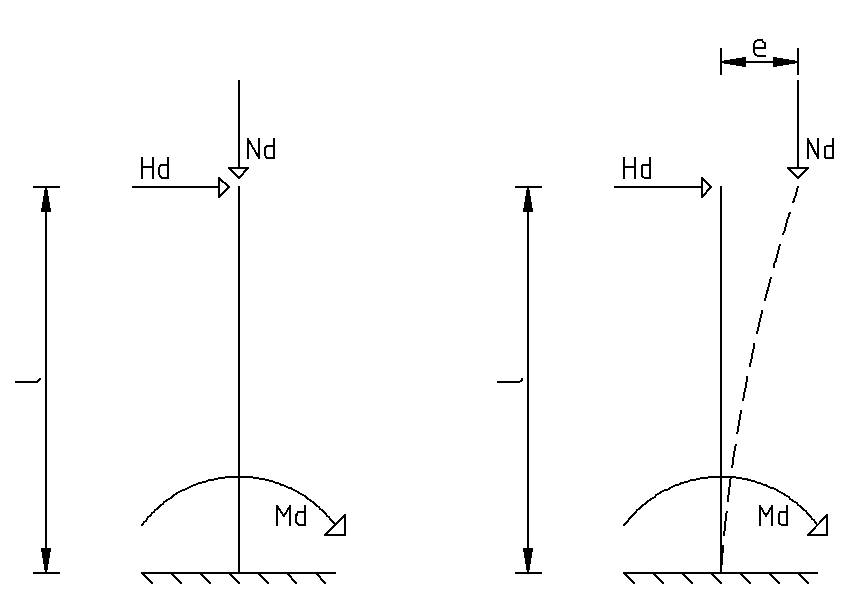
\includegraphics[width=0.5\textwidth]{Nao-linearidade-geometrica/Imagens/Efeitos-de-1a-e-2a-ordem.png}
	\end{center}
\end{figure}

	\section{Estruturas de nós fixos ou móveis}
	A \textbf{estabilidade global} de uma estrutura se dá quando \textbf{menores} forem os efeitos de 2ª ordem. Para criar condições de cálculo, as estruturas são definidas de nós fixos ou nós móveis.

\begin{itemize}
	\item \textbf{Estruturas de nós fixos}: Na verdade não são fixos, mas deslocáveis, mas os deslocamentos horizontais são muito pequenos e, por consequência, os \textbf{efeitos globais de 2ª ordem} são \textbf{desprezíveis} (<10\%). Nessas estruturas, basta considerar os \textbf{efeitos locais de 2ª ordem};

	\item \textbf{Estruturas de nós móveis}: Aquelas em que os deslocamentos horizontais \textbf{não são pequenos}, exigindo cálculo dos \textbf{efeito globais de 2ª ordem}.
\end{itemize}

Assim:

\begin{itemize}
	\item \textbf{Nós fixos}: \textbf{Não há} necessidade de se calcular efeitos globais de 2ª ordem;
	\item \textbf{Nós móveis}: \textbf{Há} necessidade de se calcular.
\end{itemize}

	\section{Coeficiente $\gamma_z$}
	O coeficiente $\gamma_z$ é um parâmetro que avalia a \textbf{estabilidade global} de uma estrutura de concreto armado de forma simples e eficiente.

Também é capaz de \textbf{estimar} os esforços globais de \textbf{2ª ordem} por uma \textbf{simples majoração} dos esforços de \textbf{1ª ordem} dos \textbf{esforços horizontais}. Valores coerentes para esse coeficiente são números um pouco maiores que 1. Porém, valores superiores a 1,2 devem ser evitados, já que as diferenças começam a ficar muito altas.

Valores entre 1,15 e 1,2 começam a aparecer diferenças de 3\% contra a segurança. Acima disso, aumentam para mais de 5\%.

De acordo com a NBR 6118, o limite para o coeficiente é 1,3 e, acima disso, a etrutura é \textbf{instável e impraticável}.

\begin{itemize}
	\item Nós fixos: $\gamma_z\leqslant$ 1,1 $\rightarrow$ Não calcula efeitos globais de 2ª ordem para carga horizontal;
	\item Nós móveis: 1,1 < $\gamma_z\leqslant$ 1,3 $\rightarrow$ Calcular os efeitos. 
\end{itemize}

Este método é válido para edifícios acima de 4 andares. Abaixo disso, \textbf{não se deve majorar} as cargas horizontais com $\gamma_z$.

O coeficiente $\gamma_z$ é: $$\gamma_z=\frac{1}{1-\frac{\Delta M_{total, d}}{M_{1, total, d}}}$$

Onde $\Delta M_{total, d}$ é a soma dos produtos de todas as forças verticais atuantes na etrutura com seus valores de cálculo pelos deslocamentos horizontais de seus respectivos pontos de aplicação, sendo: $$\Delta M_{total, d}=P_d\cdot d_{horiz}$$

$P_d$ é a soma de todas as cargas verticais ($g$ e $q$) multiplicada pela majoração do concreto, já $d_{horiz}$ é o deslocamento horizontal devido à carga horizontal (obtido no FTOOL).

$$M_{1, total, d}=\sum_{i=1}^{n} F_{d, i}\cdot H_i$$

\begin{figure}[H]
	\begin{center}
	\caption{$M_{1, total, d}$ identificado na estrutura.}
    	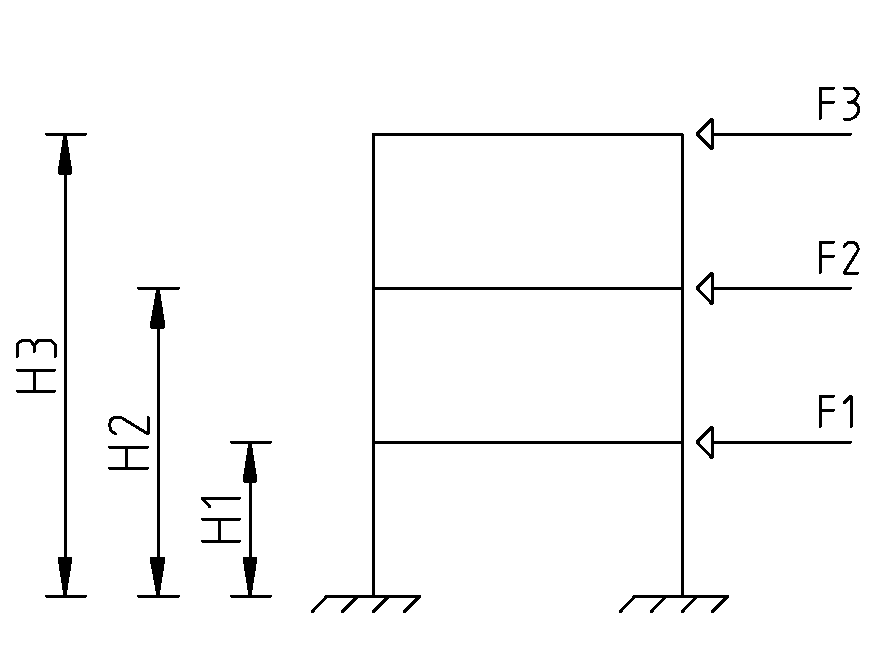
\includegraphics[width=0.5\textwidth]{Coeficiente-gamma-z/Imagens/M1-total-d.png}
	\end{center}
\end{figure}

Com isso, é possível verificar o deslocamento horizontal máximo permitido pela NBR 6118 - tabela 13.3. No topo é $H/1700$ e entre pavimentos é $H_{pisos}/850$, adotando-se coeficiente de pressão dinâmica do vento para cálculo do estado limite $\psi_1=0,30$.

	\textbf{Exercício}: Verificar o deslocamento horizontal (global e local) da estrutura abaixo em relação aos limites impostos pela NBR 6118 através do coeficiente $\gamma_z$, considerando somente a primeira combinação do ELU, sabendo-se que:

\begin{itemize}
	\item Edifício com térreo + 6 pavimentos;
	\item Altura entre pisos de 3 $m$;
	\item Carga acidental no andar-tipo de 191,52 $kN$;
	\item Carga acidental na cobertura de 63,84 $kN$;
	\item Carga permanente no andar-tipo de 1380,48 $kN$;
	\item Carga permanente na cobertura de 732,576 $kN$;
	\item Pilares de (12x40) $cm$;
	\item Quatro pilares na face do vento.
\end{itemize}

Nota: As unidades de carga descritas acima representam as reações de apoio das vigas nos pilares.

Dada a quantidade de valores para manuseio, recomenda-se para o leitor utilizar alguma planilha eletrônica para faciltar a compreensão. O primeiro passo é colocar as seguintes cargas no pórtico do presente exercício, atentando-se ao fato de que os valores de carga de vento ($H_v$) devem ser divididos pela quantidade de pilares na face do vento (4).

\begin{table}[H]
	\centering
	\caption{Valores de cota ($z$) e valores de carga de vento ($H_v$) para o presente exercício.}
	\begin{tabular}{c|c}
	\hline
	z ($m$) & $H_v$ ($kN$) \\ \hline
	3       & 19,255       \\
	6       & 22,740       \\
	9       & 25,065       \\
	12      & 26,857       \\
	15      & 28,333       \\
	18      & 29,602       \\
	21      & 15,358       \\ \hline
	\end{tabular}
\end{table}

Monta-se o pórtico no FTOOL e coloca-se 1/4 da carga de $H_v$ em cada pilar, de modo a ficar como segue:

*Inserir imagem do pórtico com as cargas

Neste exercício, o vento é considerado como efeito secundário, portanto, deve ser minorado por um coeficiente $\psi_0$, que no presente exercício equivale a 0,6 (valor para pressão dinâmica do vento para estruturas em geral, vide tabela 11.2 da NBR 6118).

Todo o exercício objetiva o encontro de $\gamma_z$ para verificar a estabilidade global do edifício e qual tipo de nó está presente na estrutura, com ele pode-se verificar se será necessário considerar os efeitos de 2ª ordem. Os parâmetros de $\gamma_z$ são $M_{1, total, d}$ e $\Delta M_{total, d}$, que são a carga horizontal final e a carga vertical, respectivamente.

O próximo passo é preencher a seguinte tabela:

\begin{table}[H]
\centering
\caption{Tabela a ser preenchida para facilitar o cálculo de $\gamma_z$.}
\label{tab:Tabela-exercicio-vento}
\begin{tabular}{c|c|c|ccc|c}
\hline
Andar & $F_d$ $minorada$ & $M_{1, total, d}$ & \multicolumn{1}{c|}{$P_d$} & \multicolumn{1}{c|}{$d_{horiz}$} & $d_{horiz}$ $minorada$ & $\Delta M_{total, d}$ \\
 & ($kN$) & ($kN\cdot cm$) & \multicolumn{1}{c|}{($kN$)} & \multicolumn{1}{c|}{($cm$) (FTOOL)} & ($cm$) & ($kN\cdot cm$) \\ \hline
1 &  &  & \multicolumn{1}{c|}{} & \multicolumn{1}{c|}{} &  &  \\
2 &  &  & \multicolumn{1}{c|}{} & \multicolumn{1}{c|}{} &  &  \\
3 &  &  & \multicolumn{1}{c|}{} & \multicolumn{1}{c|}{} &  &  \\
4 &  &  & \multicolumn{1}{c|}{} & \multicolumn{1}{c|}{} &  &  \\
5 &  &  & \multicolumn{1}{c|}{} & \multicolumn{1}{c|}{} &  &  \\
6 &  &  & \multicolumn{1}{c|}{} & \multicolumn{1}{c|}{} &  &  \\
7 &  &  & \multicolumn{1}{c|}{} & \multicolumn{1}{c|}{} &  &  \\ \hline
Total &  &  &  &  &  &  \\ \cline{1-1} \cline{3-3} \cline{7-7} 
\end{tabular}
\end{table}

Onde $F_{d, minorada}$ é a carga de vento minorada (já que o respectivo efeito é considerado secundário; é a minoração de $H_v$), $M_{1, total, d}$ é o momento fletor que a carga horizontal causa na estrutura, $Pd$ é a carga vertical atuante na estrutura ($g+q$) unitária de cada andar, $d_{horiz}$ é o deslocamento horizontal causado pela carga horizontal (obtido no FTOOL), $d_{horiz}\;minorada$ é o deslocamento horizontal causado pela carga horizontal minorada (novamente, o efeito dos ventos está sendo considerado como secundário no exercício) e $\Delta M_{total, d}$ é o momento fletor gerado pelo deslocamento horizontal causado pelas cargas verticais. O 7º pavimento é a cobertura.

Calcula-se $F_{d, minorada}$ pela equação:
\begin{equation}F_{d, minorada}=1,4\cdot\psi_0\cdot H_v\end{equation}

Por exemplo, para o 1º e 2º andar, respectivamente: $$F_{d, minorada}=1,4\cdot 0,6\cdot 19,255\;kN=16,1742\;kN$$, $$F_{d, minorada}=1,4\cdot 0,6\cdot 22,740\;kN=19,1016\;kN$$

Preenchendo a respectiva coluna na Tabela~\ref{tab:Tabela-exercicio-vento}, tem-se:

\begin{table}[H]
\centering
\begin{tabular}{c|c|c|ccc|c}
\hline
Andar & $F_d$ $minorado$ & $M_{1, total, d}$ & \multicolumn{1}{c|}{$P_d$} & \multicolumn{1}{c|}{$d_{horiz}$} & $d_{horiz}$ $minorada$ & $\Delta M_{total, d}$ \\
 & ($kN$) & ($kN\cdot cm$) & \multicolumn{1}{c|}{($kN$)} & \multicolumn{1}{c|}{($cm$) (FTOOL)} & ($cm$) & ($kN\cdot cm$) \\ \hline
1 & 16,1742 &  & \multicolumn{1}{c|}{} & \multicolumn{1}{c|}{} &  &  \\
2 & 19,1016 &  & \multicolumn{1}{c|}{} & \multicolumn{1}{c|}{} &  &  \\
3 & 21,0546 &  & \multicolumn{1}{c|}{} & \multicolumn{1}{c|}{} &  &  \\
4 & 22,5599 &  & \multicolumn{1}{c|}{} & \multicolumn{1}{c|}{} &  &  \\
5 & 23,7997 &  & \multicolumn{1}{c|}{} & \multicolumn{1}{c|}{} &  &  \\
6 & 24,8657 &  & \multicolumn{1}{c|}{} & \multicolumn{1}{c|}{} &  &  \\
7 & 12,9007 &  & \multicolumn{1}{c|}{} & \multicolumn{1}{c|}{} &  &  \\ \hline
Total &  &  &  &  &  &  \\ \cline{1-1} \cline{3-3} \cline{7-7} 
\end{tabular}
\end{table}

Agora, pode-se calcular o momento fletor ($M_{1, total, d}$) causado por cada força horizontal ($F_{d, minorada}$) em relação à base do edifício. Para o 1º e 2º andar, tem-se, respectivamente:
$$M_{1, total, d}=F_{d, minorada}\cdot z=16,1742\;kN\cdot 300\;cm=4852,26\;kN\cdot cm$$
$$M_{1, total, d}=F_{d, minorada}\cdot z=19,1016\;kN\cdot 600\;cm=11460,96\;kN\cdot cm$$

Note que a cota ($z$) é a altura que o respectivo pavimento está da base. Preenchendo a respectiva coluna na Tabela~\ref{tab:Tabela-exercicio-vento}, tem-se:

\begin{table}[H]
\centering
\begin{tabular}{c|c|c|ccc|c}
\hline
Andar & $F_d$ $minorada$ & $M_{1, total, d}$ & \multicolumn{1}{c|}{$P_d$} & \multicolumn{1}{c|}{$d_{horiz}$} & $d_{horiz}$ $minorada$ & $\Delta M_{total, d}$ \\
 & ($kN$) & ($kN\cdot cm$) & \multicolumn{1}{c|}{($kN$)} & \multicolumn{1}{c|}{($cm$) (FTOOL)} & ($cm$) & ($kN\cdot cm$) \\ \hline
1 & 16,1742 & 4852,26 & \multicolumn{1}{c|}{} & \multicolumn{1}{c|}{} &  &  \\
2 & 19,1016 & 11460,96 & \multicolumn{1}{c|}{} & \multicolumn{1}{c|}{} &  &  \\
3 & 21,0546 & 18949,14 & \multicolumn{1}{c|}{} & \multicolumn{1}{c|}{} &  &  \\
4 & 22,5599 & 27071,88 & \multicolumn{1}{c|}{} & \multicolumn{1}{c|}{} &  &  \\
5 & 23,7997 & 35699,55 & \multicolumn{1}{c|}{} & \multicolumn{1}{c|}{} &  &  \\
6 & 24,8657 & 44758,26 & \multicolumn{1}{c|}{} & \multicolumn{1}{c|}{} &  &  \\
7 & 12,9007 & 27091,47 & \multicolumn{1}{c|}{} & \multicolumn{1}{c|}{} &  &  \\ \hline
Total &  & 169883,53 &  &  &  &  \\ \cline{1-1} \cline{3-3} \cline{7-7} 
\end{tabular}
\end{table}

A carga vertical $P_d$ é a mesma para todos os pavimentos tipo, sendo: $$P_d=g+q=1,4\cdot1380,48\;kN+1,4\cdot191,52\;kN=2200,8\;kN$$

A carga vertical $P_d$ para a cobertura é: $$P_d=g+q=1,4\cdot 732,576\;kN+1,4\cdot63,84\;kN=1114,9824\;kN$$

Preenchendo a respectiva coluna na Tabela~\ref{tab:Tabela-exercicio-vento}, tem-se:

\begin{table}[H]
\centering
\begin{tabular}{c|c|c|ccc|c}
\hline
Andar & $F_d$ $minorada$ & $M_{1, total, d}$ & \multicolumn{1}{c|}{$P_d$} & \multicolumn{1}{c|}{$d_{horiz}$} & $d_{horiz}$ $minorada$ & $\Delta M_{total, d}$ \\
 & ($kN$) & ($kN\cdot cm$) & \multicolumn{1}{c|}{($kN$)} & \multicolumn{1}{c|}{($cm$) (FTOOL)} & ($cm$) & ($kN\cdot cm$) \\ \hline
1 & 16,1742 & 4852,26 & \multicolumn{1}{c|}{2200,800} & \multicolumn{1}{c|}{} &  &  \\
2 & 19,1016 & 11460,96 & \multicolumn{1}{c|}{2200,800} & \multicolumn{1}{c|}{} &  &  \\
3 & 21,0546 & 18949,14 & \multicolumn{1}{c|}{2200,800} & \multicolumn{1}{c|}{} &  &  \\
4 & 22,5599 & 27071,88 & \multicolumn{1}{c|}{2200,800} & \multicolumn{1}{c|}{} &  &  \\
5 & 23,7997 & 35699,55 & \multicolumn{1}{c|}{2200,800} & \multicolumn{1}{c|}{} &  &  \\
6 & 24,8657 & 44758,26 & \multicolumn{1}{c|}{2200,800} & \multicolumn{1}{c|}{} &  &  \\
7 & 12,9007 & 27091,47 & \multicolumn{1}{c|}{1114,9824} & \multicolumn{1}{c|}{} &  &  \\ \hline
Total &  & 169883,53 &  &  &  &  \\ \cline{1-1} \cline{3-3} \cline{7-7} 
\end{tabular}
\end{table}

O valor de $d_{horiz}$ é obtido através do software livre FTOOL. Preenchendo a respectiva coluna na Tabela~\ref{tab:Tabela-exercicio-vento}, tem-se:

\begin{table}[H]
\centering
\begin{tabular}{c|c|c|ccc|c}
\hline
Andar & $F_d$ $minorada$ & $M_{1, total, d}$ & \multicolumn{1}{c|}{$P_d$} & \multicolumn{1}{c|}{$d_{horiz}$} & $d_{horiz}$ $minorada$ & $\Delta M_{total, d}$ \\
 & ($kN$) & ($kN\cdot cm$) & \multicolumn{1}{c|}{($kN$)} & \multicolumn{1}{c|}{($cm$) (FTOOL)} & ($cm$) & ($kN\cdot cm$) \\ \hline
1 & 16,1742 & 4852,26 & \multicolumn{1}{c|}{2200,800} & \multicolumn{1}{c|}{0,3228} &  &  \\
2 & 19,1016 & 11460,96 & \multicolumn{1}{c|}{2200,800} & \multicolumn{1}{c|}{0,7735} &  &  \\
3 & 21,0546 & 18949,14 & \multicolumn{1}{c|}{2200,800} & \multicolumn{1}{c|}{1,1816} &  &  \\
4 & 22,5599 & 27071,88 & \multicolumn{1}{c|}{2200,800} & \multicolumn{1}{c|}{1,5184} &  &  \\
5 & 23,7997 & 35699,55 & \multicolumn{1}{c|}{2200,800} & \multicolumn{1}{c|}{1,7743} &  &  \\
6 & 24,8657 & 44758,26 & \multicolumn{1}{c|}{2200,800} & \multicolumn{1}{c|}{1,9440} &  &  \\
7 & 12,9007 & 27091,47 & \multicolumn{1}{c|}{1114,9824} & \multicolumn{1}{c|}{2,0326} &  &  \\ \hline
Total &  & 169883,53 &  &  &  &  \\ \cline{1-1} \cline{3-3} \cline{7-7} 
\end{tabular}
\end{table}

O valor contido na tabela de $d_{horiz}$ foi obtido no FTOOL a partir da carga $H_v$ (não minorada). Para obtermos $d_{horiz, minorada}$, deve-se minorar $d_{horiz}$ pelos mesmos fatores utilizados para minorar $H_v$. Para o 1º e 2º andar, tem-se:
$$d_{horiz, minorada}=1,4\cdot\psi_0\cdot d_{horiz}=1,4\cdot0,6\cdot 0,3228\;cm=0,2712\;cm$$ $$d_{horiz, minorada}=1,4\cdot\psi_0\cdot d_{horiz}=1,4\cdot0,6\cdot 0,7735\;cm=0,6497\;cm$$

Preenchendo a respectiva coluna na Tabela~\ref{tab:Tabela-exercicio-vento}, tem-se:

\begin{table}[H]
\centering
\begin{tabular}{c|c|c|ccc|c}
\hline
Andar & $F_d$ $minorada$ & $M_{1, total, d}$ & \multicolumn{1}{c|}{$P_d$} & \multicolumn{1}{c|}{$d_{horiz}$} & $d_{horiz}$ $minorada$ & $\Delta M_{total, d}$ \\
 & ($kN$) & ($kN\cdot cm$) & \multicolumn{1}{c|}{($kN$)} & \multicolumn{1}{c|}{($cm$) (FTOOL)} & ($cm$) & ($kN\cdot cm$) \\ \hline
1 & 16,1742 & 4852,26 & \multicolumn{1}{c|}{2200,800} & \multicolumn{1}{c|}{0,3228} & 0,2712 &  \\
2 & 19,1016 & 11460,96 & \multicolumn{1}{c|}{2200,800} & \multicolumn{1}{c|}{0,7735} & 0,6497 &  \\
3 & 21,0546 & 18949,14 & \multicolumn{1}{c|}{2200,800} & \multicolumn{1}{c|}{1,1816} & 0,9925 &  \\
4 & 22,5599 & 27071,88 & \multicolumn{1}{c|}{2200,800} & \multicolumn{1}{c|}{1,5184} & 1,2755 &  \\
5 & 23,7997 & 35699,55 & \multicolumn{1}{c|}{2200,800} & \multicolumn{1}{c|}{1,7743} & 1,4904 &  \\
6 & 24,8657 & 44758,26 & \multicolumn{1}{c|}{2200,800} & \multicolumn{1}{c|}{1,9440} & 1,6330 &  \\
7 & 12,9007 & 27091,47 & \multicolumn{1}{c|}{1114,9824} & \multicolumn{1}{c|}{2,0326} & 1,7074 &  \\ \hline
Total &  & 169883,53 &  &  &  &  \\ \cline{1-1} \cline{3-3} \cline{7-7} 
\end{tabular}
\end{table}

A última coluna da tabela, $\Delta M_{total, d}$, que é o momento fletor causado pela carga vertical vezes a excentricidade causada pela carga horizontal, é, para o 1º e 2º andar, respectivamente:
$$\Delta M_{total, d}=P_d\cdot d_{horiz, minorada}=2200,800\;kN\cdot0,2712\;cm=596,7513\;kN\cdot cm$$
$$\Delta M_{total, d}=P_d\cdot d_{horiz, minorada}=2200,800\;kN\cdot0,6497\;cm=1429,9478\;kN\cdot cm$$

Preenchendo a respectiva coluna na Tabela~\ref{tab:Tabela-exercicio-vento}, tem-se:

\begin{table}[H]
\centering
\begin{tabular}{c|c|c|ccc|c}
\hline
 & $F_d$ $minorada$ & $M_{1, total, d}$ & \multicolumn{1}{c|}{$P_d$} & \multicolumn{1}{c|}{$d_{horiz}$} & $d_{horiz}$ $minorada$ & $\Delta M_{total, d}$ \\
 & ($kN$) & ($kN\cdot cm$) & \multicolumn{1}{c|}{($kN$)} & \multicolumn{1}{c|}{($cm$) (FTOOL)} & ($cm$) & ($kN\cdot cm$) \\ \hline
1 & 16,1742 & 4852,26 & \multicolumn{1}{c|}{2200,800} & \multicolumn{1}{c|}{0,3228} & 0,2712 & 596,7513 \\
2 & 19,1016 & 11460,96 & \multicolumn{1}{c|}{2200,800} & \multicolumn{1}{c|}{0,7735} & 0,6497 & 1429,9478 \\
3 & 21,0546 & 18949,14 & \multicolumn{1}{c|}{2200,800} & \multicolumn{1}{c|}{1,1816} & 0,9925 & 2184,3908 \\
4 & 22,5599 & 27071,88 & \multicolumn{1}{c|}{2200,800} & \multicolumn{1}{c|}{1,5184} & 1,2755 & 2807,0236 \\
5 & 23,7997 & 35699,55 & \multicolumn{1}{c|}{2200,800} & \multicolumn{1}{c|}{1,7743} & 1,4904 & 3280,0987 \\
6 & 24,8657 & 44758,26 & \multicolumn{1}{c|}{2200,800} & \multicolumn{1}{c|}{1,9440} & 1,6330 & 3593,8184 \\
7 & 12,9007 & 27091,47 & \multicolumn{1}{c|}{1114,9824} & \multicolumn{1}{c|}{2,0326} & 1,7074 & 1903,6990 \\ \hline
Total &  & 169883,53 &  &  &  & 15795,7296 \\ \cline{1-1} \cline{3-3} \cline{7-7} 
\end{tabular}
\end{table}

Agora, pode-se calcular o valor de $\gamma_z$ para verificarmos o tipo de nó presente na estrutura.
$$\gamma_z=\frac{1}{1-\frac{\Delta M_{total, d}}{M_{1, total, d}}}=\frac{1}{1-\frac{15795,7296\;kN}{169883,53\;kN}}\approx1,1025$$

Portanto, o tipo de nó é móvel ($1,1<\gamma_z\leqslant1,3$). Nós móveis obriga a definição dos efeitos de 2ª ordem para as cargas horizontais. Para isso, a NBR 6118 permite majorar a carga de vento com a equação:
\begin{equation}H_{v2}=H_v\cdot0,95\cdot\gamma_z\end{equation}

Onde $H_{v2}$ é a nova carga de vento majorada em $kN$, $H_v$ é a carga de vento nos nós da estrutura em $kN$ e $\gamma_z$ é o coeficiente de estabilidade global (adimensional).

Essa nova carga horizontal ($H_{v2}/4$) deve ser colocada no lugar da antiga ($H_v/4$) no FTOOL objetivando encontrar novos deslocamentos horizontais. Pode-se, então, montar a seguinte tabela para facilitar os cálculos:

\begin{table}[H]
\centering
\caption{Tabela a ser preenchida para verificação de deslocamento horizontal em nós móveis.}
\label{tab:Tabela-exercicio-deslocamento-nos-moveis}
\begin{tabular}{c|c|c|c|c|c}
\hline
\begin{tabular}[c]{@{}c@{}}z\\ ($m$)\end{tabular} & \begin{tabular}[c]{@{}c@{}}$H_{v2}$\\ ($kN$)\end{tabular} & \begin{tabular}[c]{@{}c@{}}$\frac{H_{v2}}{4}$\\ ($kN$)\end{tabular} & \begin{tabular}[c]{@{}c@{}}$d_{horiz, 2}$\\ FTOOL ($cm$)\end{tabular} & \begin{tabular}[c]{@{}c@{}}$d_{horiz, 2}\cdot\psi_1$\\ ($cm$)\end{tabular} & \begin{tabular}[c]{@{}c@{}}$\Delta_{desloc, 2}$\\ ($cm$)\end{tabular} \\ \hline
3                                                 & 20,1674                                                                      & 5,0419                                                              & 0,3448                                                                &                                                                            &                                                                    \\
6                                                 & 23,8176                                                                      & 5,9544                                                              & 0,8263                                                                &                                                                            &                                                                    \\
9                                                 & 26,2527                                                                      & 6,5632                                                              & 1,2622                                                                &                                                                            &                                                                    \\
12                                                & 28,1296                                                                      & 7,0324                                                              & 1,6221                                                                &                                                                            &                                                                    \\
15                                                & 29,6756                                                                      & 7,4189                                                              & 1,8954                                                                &                                                                            &                                                                    \\
18                                                & 31,0047                                                                      & 7,7512                                                              & 2,0767                                                                &                                                                            &                                                                    \\
21                                                & 16,0857                                                                      & 4,0214                                                              & 2,1713                                                                &                                                                            &                                                                    \\ \hline
\end{tabular}
\end{table}

O coeficiente $\psi_1$ na penúltima coluna é o valor de pressão dinâmica do vento nas estruturas em geral (0,3). O valor do produto ($d_{horiz, 2}\cdot\psi_1$) diz respeito ao \textbf{deslocamento global} da estrutura. O valor de $\Delta_{desloc, 2}$ diz respeito a variação de deslocamento entre um pavimento e o logo abaixo, ou seja, o \textbf{deslocamento local}. O referido produto para o 6º pavimento e cobertura são, respectivamente:
$$d_{horiz}\cdot\psi_1=2,0767\cdot0,3=0,6230\;cm$$
$$d_{horiz}\cdot\psi_1=2,1713\cdot0,3=0,6513\;cm$$

O valor de deslocamento local de cada pavimento deve ser obtido da seguinte forma:
\begin{equation}{\Delta_{desloc, 2}}_i={(d_{horiz}\cdot\psi_1)}_i-{(d_{horiz}\cdot\psi_1)}_{i-1}\end{equation}

O valor de $\Delta_{desloc, 2}$ para a cobertura é, portanto: $$\Delta_{desloc, 2}=0,6513-0,6230=0,0283\;cm$$

Completanto a Tabela~\ref{tab:Tabela-exercicio-deslocamento-nos-moveis}, tem-se:

\begin{table}[H]
\centering
\begin{tabular}{c|c|c|c|c|c}
\hline
\begin{tabular}[c]{@{}c@{}}z\\ ($m$)\end{tabular} & \begin{tabular}[c]{@{}c@{}}$H_v\cdot0,95\cdot\gamma_z$\\ ($kN$)\end{tabular} & \begin{tabular}[c]{@{}c@{}}$\frac{H_{v2}}{4}$\\ ($kN$)\end{tabular} & \begin{tabular}[c]{@{}c@{}}$d_{horiz, 2}$\\ FTOOL ($cm$)\end{tabular} & \begin{tabular}[c]{@{}c@{}}$d_{horiz, 2}\cdot\phi_1$\\ ($cm$)\end{tabular} & \begin{tabular}[c]{@{}c@{}}$\Delta desloc 2$\\ ($cm$)\end{tabular} \\ \hline
3                                                 & 20,1674                                                                      & 5,0419                                                              & 0,3448                                                                & 0,10344                                                                    & 0,1034                                                             \\
6                                                 & 23,8176                                                                      & 5,9544                                                              & 0,8263                                                                & 0,24789                                                                    & 0,1445                                                             \\
9                                                 & 26,2527                                                                      & 6,5632                                                              & 1,2622                                                                & 0,37866                                                                    & 0,1308                                                             \\
12                                                & 28,1296                                                                      & 7,0324                                                              & 1,6221                                                                & 0,48663                                                                    & 0,1080                                                             \\
15                                                & 29,6756                                                                      & 7,4189                                                              & 1,8954                                                                & 0,56862                                                                    & 0,0820                                                             \\
18                                                & 31,0047                                                                      & 7,7512                                                              & 2,0767                                                                & 0,62301                                                                    & 0,0544                                                             \\
21                                                & 16,0857                                                                      & 4,0214                                                              & 2,1713                                                                & 0,65139                                                                    & 0,0283                                                             \\ \hline
\end{tabular}
\end{table}

Nota: Alguns valores podem ficar bem próximos, já que foram feitos em planilha eletrônica. O importante é entender o processo lógico por trás do método.

Por fim, verifica-se se os deslocamentos estão dentro do aceitável pela NBR 6118, que são:

\begin{itemize}
	\item Para o topo: $H/1700$, onde $H$ é a cota da cobertura (verificação global);
	\item Para entre pisos: $H_{pisos}/850$, onde $H_{pisos}$ é a altura piso a piso (verificação local).
\end{itemize}

Para o topo, tem-se: $$H/1700=2100\;cm/1700\approx1,2553\;cm>0,6513\;cm\;(OK)$$
Para o entre pisos, checa-se com o maior valor de $\Delta_{desloc, 2}$ presente na Tabela~\ref{tab:Tabela-exercicio-deslocamento-nos-moveis}. Tem-se: $$H_{pisos}/850=300\;cm/850\approx0,3529\;cm>0,1445\;cm\;(OK)$$

Os deslocamentos global e local atendem às exigencias da NBR 6118.

	\section{Pilar intermediário, de extremidade e de canto}
	A classificação de pilares tem como objetivo considerar as diferentes situações de projeto e de cálculo, em relação aos esforços solicitantes em que cada um desses pilares se enquadra.

\begin{itemize}
	\item \textbf{Pilar intermediário}: Estão submetidos preponderantemente às forças axiais de compressão, pois os módulos dos momentos fletores são de pequena intensidade em relação às ações verticais apenas. Portanto, na situação de projeto, admite-se o pilar intermediário submetido a uma compressão centrada, isto é, a excentricidade inicial é considerada igual a zero para o dimensionamento das áreas das armaduras;

	\begin{figure}[H]
		\begin{center}
		\caption{Vista em planta de um pilar intermediário.}
    		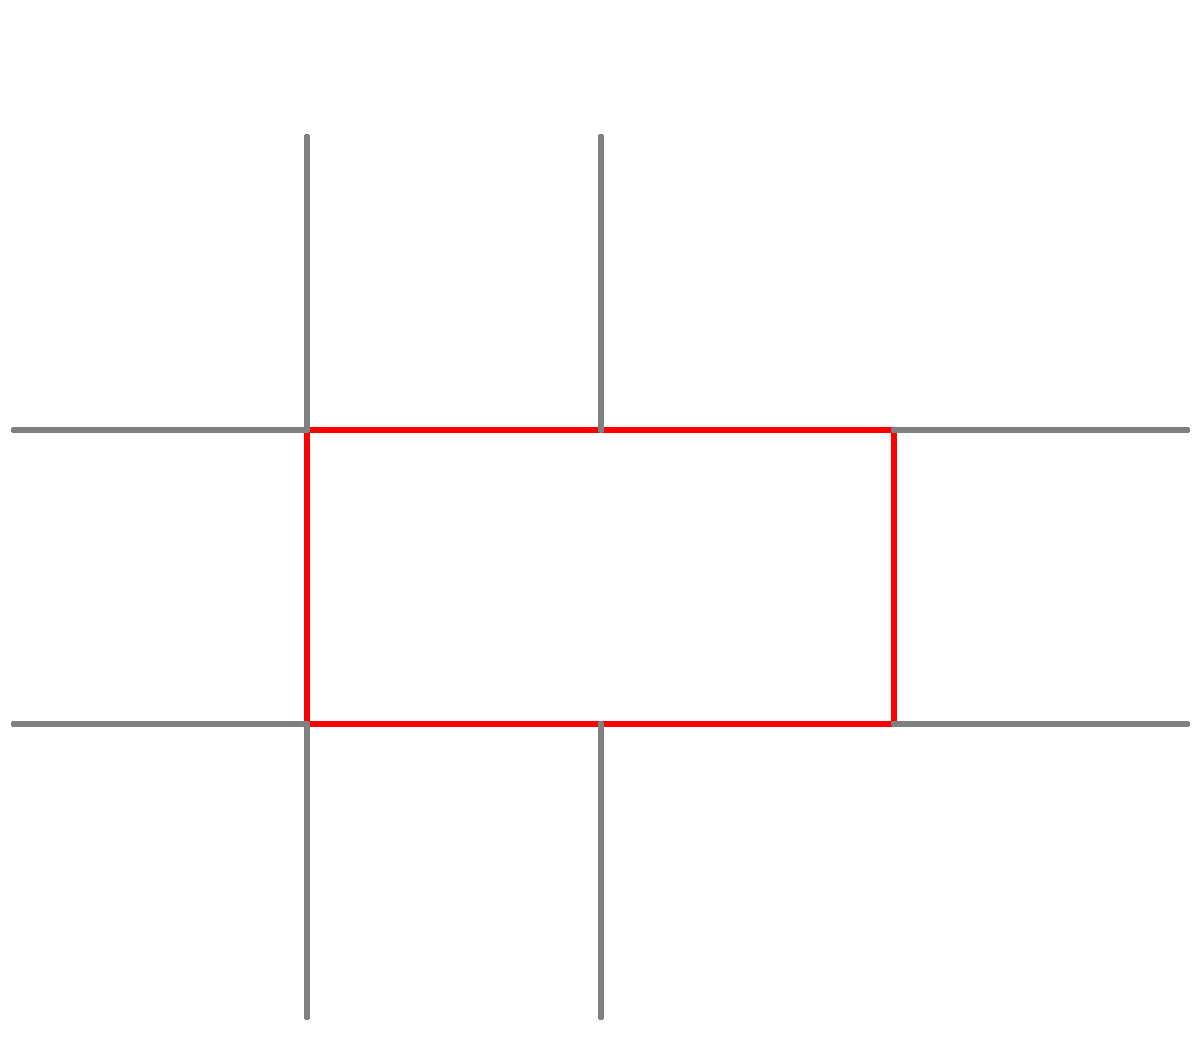
\includegraphics[width=0.3\textwidth]{Pilar-intermediario-de-extremidade-e-de-canto/Imagens/Pilar-intermediario.png}
		\end{center}
	\end{figure}

	\item \textbf{Pilar de extremidade}: Ficam posicionados nas bordas das edificações, sendo também chamados de laterais ou de borda. O termo "pilar de extremidade" advém do fato do pilar ser extremo para uma viga, aquela que não tem continuidade sobre o pilar. Além de estarem submetidos às forças normais de compressão, também estão sujeitos à ação de momentos transmitidos pelas vigas que têm suas extremidades externas nesses pilares. Portanto, na situação de projeto, admite-se o pilar de extremidade submetido à flexão normal composta, considerando-se excentricidade inicial segundo uma das coordenadas locais da seção tranversal do pilar;

	\begin{figure}[H]
		\begin{center}
		\caption{Vista em planta de um pilar de extremidade.}
    		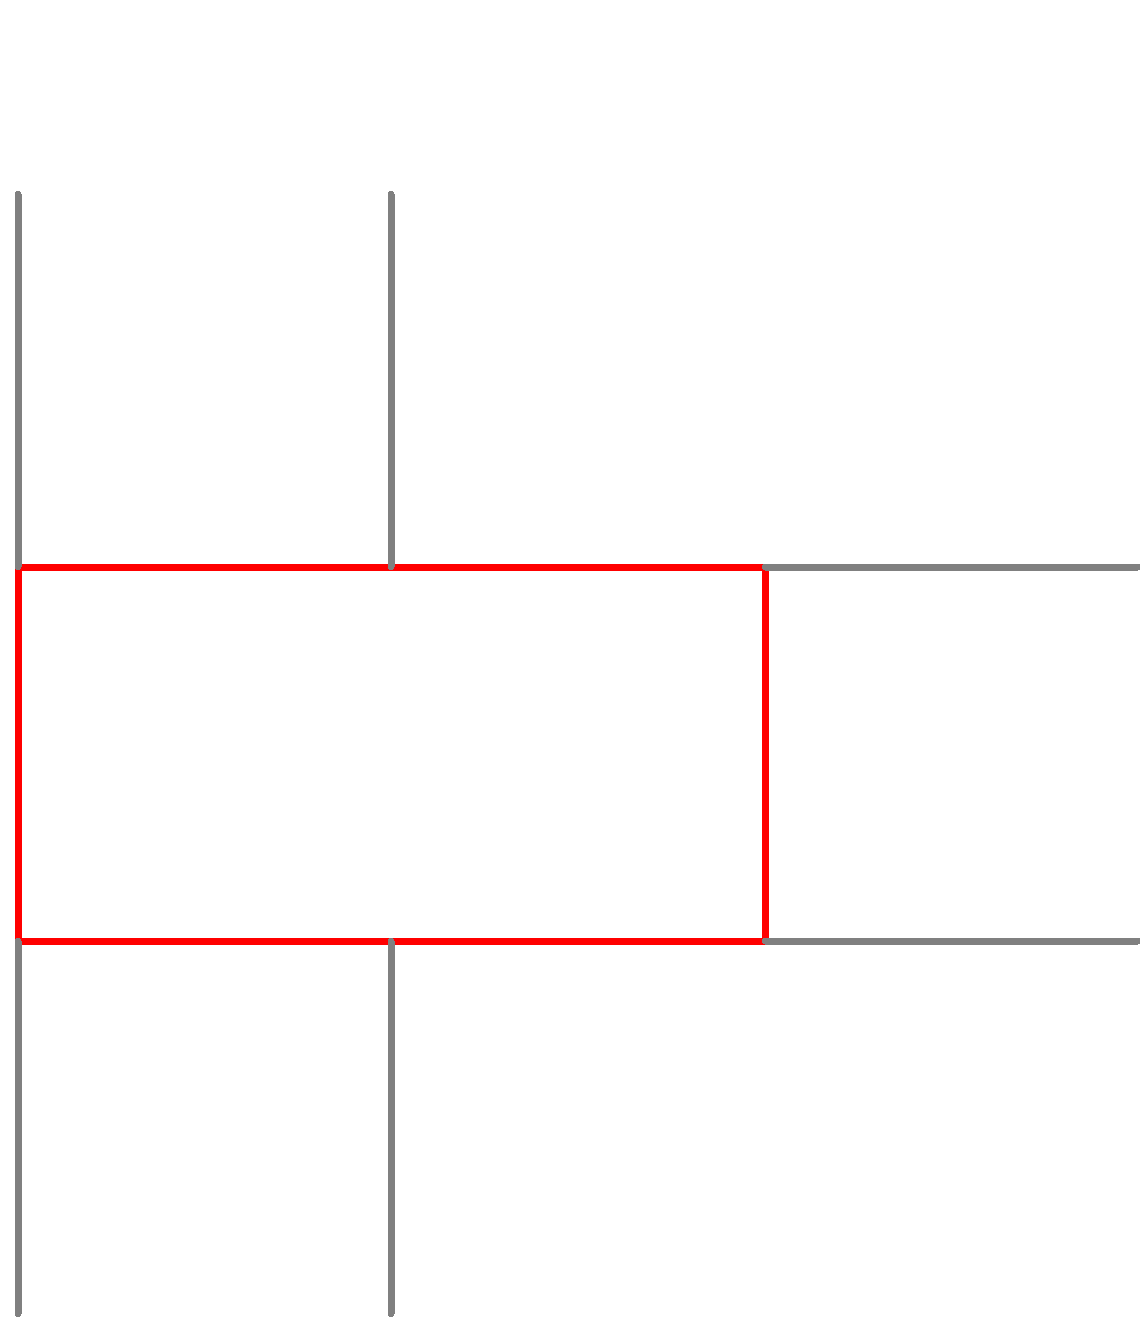
\includegraphics[width=0.2\textwidth]{Pilar-intermediario-de-extremidade-e-de-canto/Imagens/Pilar-de-extremidade.png}
		\end{center}
	\end{figure}

	\item \textbf{Pilar de canto}: Além da força normal de compressão atuante, consideram-se os momentos transmitidos pelas vigas, cujos planos médios são perpendiculares às faces dos pilares, e são interrompidas nas bordas do pilar. Na situação de projeto, considera-se o pilar de canto submetido à flexão obliqua composta, com excentricidades iniciais segundo os eixos coordenados locais.

	\begin{figure}[H]
		\begin{center}
		\caption{Vista em planta de um pilar de canto.}
    		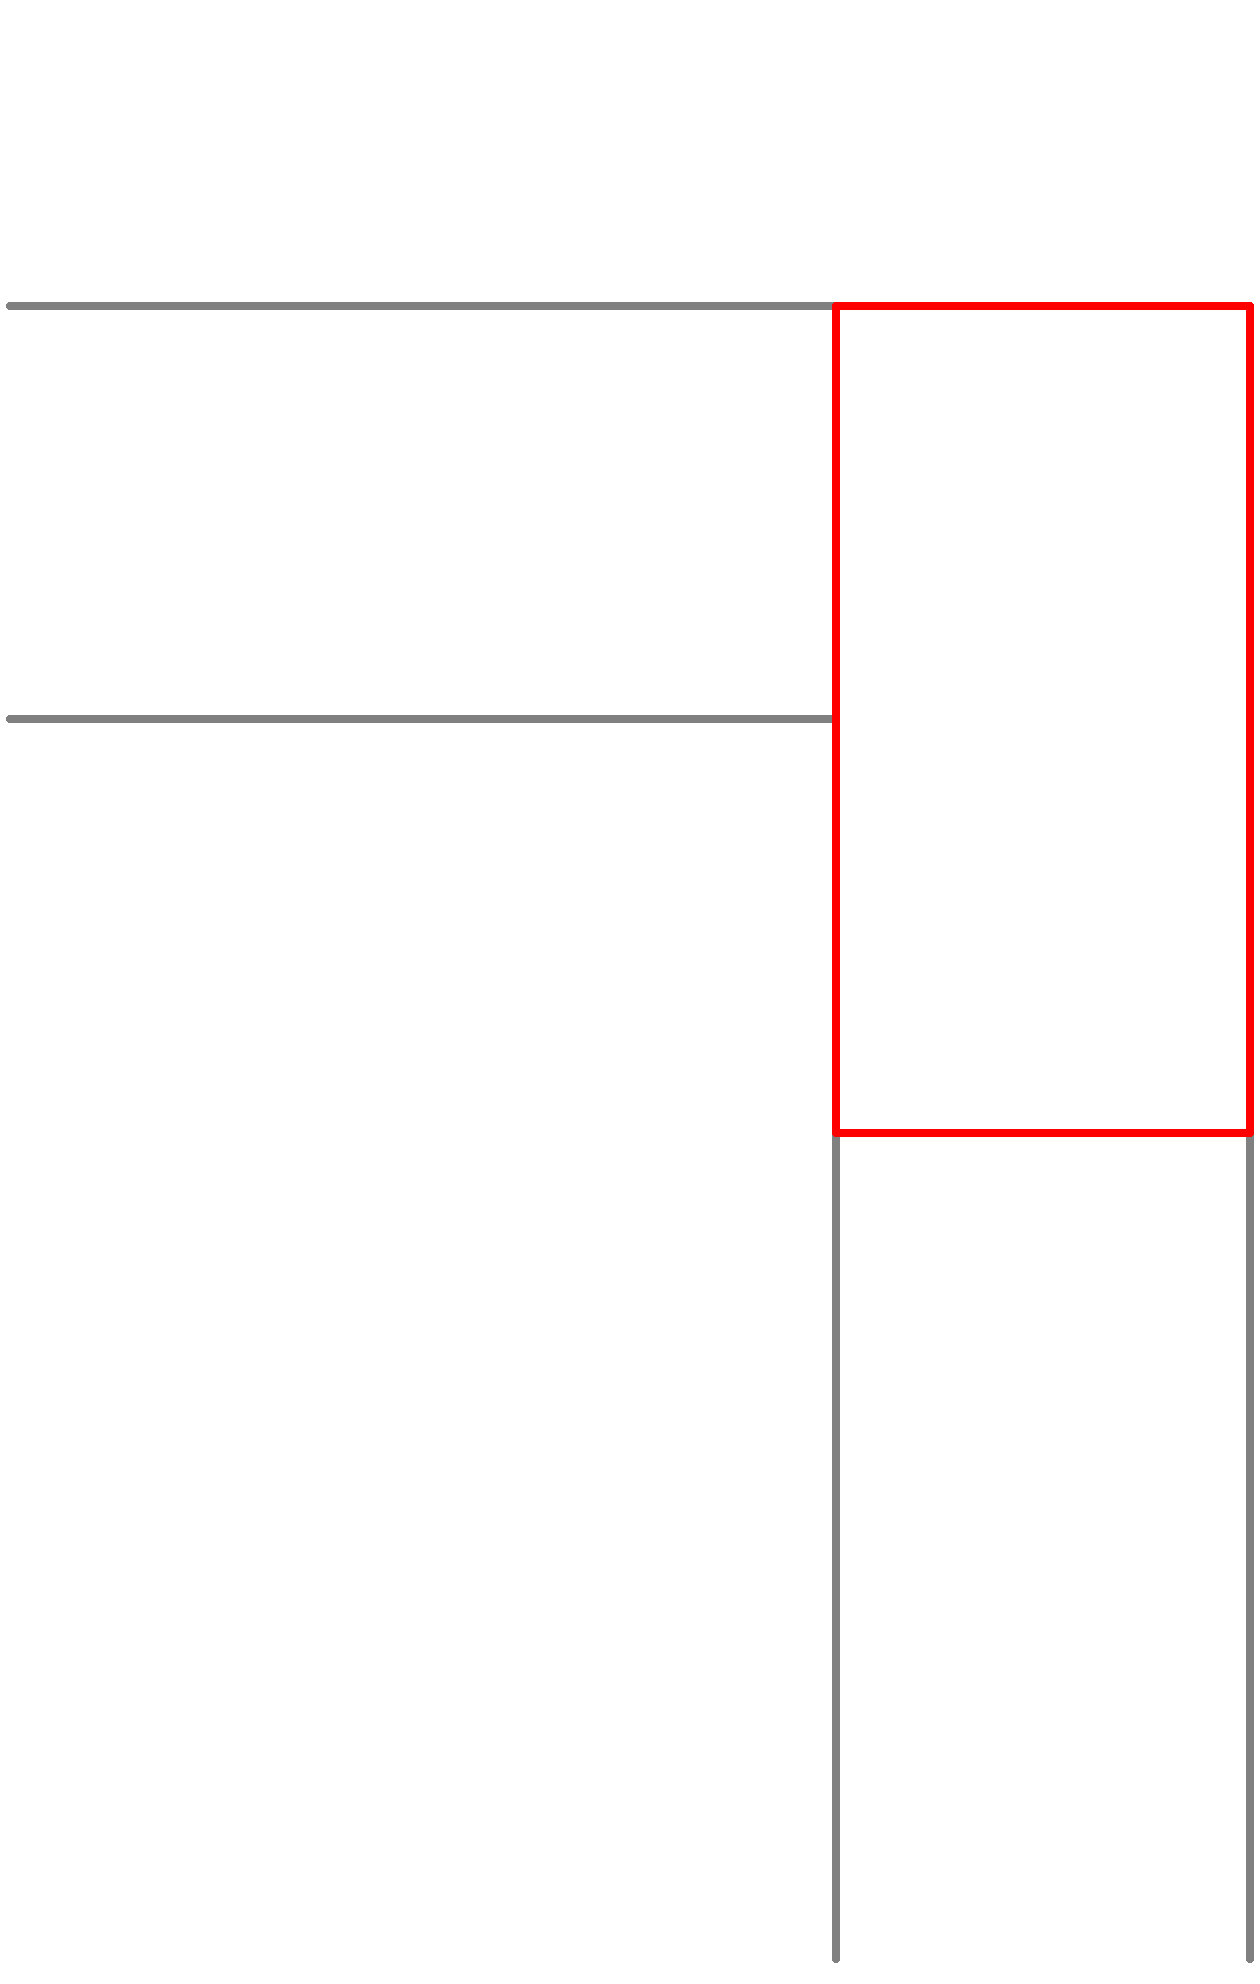
\includegraphics[width=0.2\textwidth]{Pilar-intermediario-de-extremidade-e-de-canto/Imagens/Pilar-de-canto.png}
		\end{center}
	\end{figure}

\end{itemize}

	\section{Pré-dimensionamento da seção do pilar}
	Para definição da seção de cada tipo de pilar, utiliza-se o \textbf{pilar do térreo}, que é o que recebe maior carga entre todos os pilares e mantém-se essa seção até o último andar.

Sabendo-se as cargas acima do pilar (variável e permanente), $N_d$ será o valor da reação de apoio com as majorações necessárias. Se as cargas forem pré-dimensionadas, é possível também pré-dimensionar a seção dos pilares em função do tipo de pilar e para aço CA-50.

\begin{itemize}
	\item \textbf{Pilar intermediário}:
		\begin{equation}A_c=\frac{N_d}{0,5\cdot f_{ck}+0,4}\end{equation}
	\item \textbf{Pilar de extremidade} e \textbf{pilar de canto}:
		\begin{equation}A_c=\frac{1,5\cdot N_d}{0,5\cdot f_{ck}+0,4}\end{equation}
\end{itemize}

Onde $A_c$ é a área da seção transversal do pilar, $N_d$ é a força normal de cálculo e $f_{ck}$ é a resistência característica do concreto à compressão.

Lembrando: Sem ter a seção do pilar ainda definida, $N_d$ é calculada apenas com a majoração do concreto:
\begin{equation}N_d=\gamma_f\cdot N_k=1,4\cdot N_k\end{equation}

Sabendo-se a área de concreto, devemos consultar a NBR 6118 para saber a área mínima a ser utilizada e também a medida mínima da menor dimensão do pilar.

Item 13.2.3 - A seção transversal de pilares e pilar-paredes maciços, qualquer que seja sua forma, não pode apresentar dimensão menor que 19 $cm$. Em casos especiais, permite-se considerações de dimensões entre 19 e 14 $cm$, desde que se multipliquem os esforços solicitantes de cálculo a serem considerados no dimensionamento por um coeficiente adicional $\gamma_n$, de acordo com o indicado na tabela 13.1 e seção 11 da norma. Em qualquer caso, \textbf{não se permite} pilar com seção transversal de área inferior a 360 ${cm}^2$.

*inserir tabela

A maior dimensão da seção do pilar deve ser sempre em \textbf{múltiplos de 5 $cm$}.

Sabendo-se o valor de $\gamma_n$, pode-se calcular o valor de $N_d$:
\begin{equation}N_d=\gamma_n\cdot\gamma_f\cdot N_k\end{equation}

Exercício: Pré-dimensionar a seção de um pilar intermediário, sabendo-se que: Aço CA-50; Concreto C25 ($f_{ck}=25\;MPa=250\;kgf/{cm}^2$); $\gamma_f=1,4$; $q=14051,52\;kgf$ e $g=144529,92\;kgf$.

Calcular $b=16\;cm$ e depois $b=19\;cm$. Lembre-se que não queremos pilar-parede (onde $h=5\cdot b$).

Para o pilar com $b=16\;cm$, tem-se:
$$A_c=\frac{N_d}{0,5\cdot f_{ck}+0,4}=\frac{1,4\cdot1,15\cdot(14051,52+144529,92)}{0,5\cdot250+0,4}\approx2036,0137\;{cm}^2$$

Com essa área, checa-se se não é um pilar parede (limite de $5\cdot b=5\cdot16\;cm=80\;cm$):
$$h=\frac{A_c}{b}=\frac{2036,0137\;{cm}^2}{16\;cm}\approx127,2508\;cm\approx130\;cm$$

O valor de $h$ ultrapassou o limite e, dessa forma, o pilar é considerado pilar-parede.

Para o pilar com $b=19\;cm$, tem-se:
$$A_c=\frac{N_d}{0,5\cdot f_{ck}+0,4}=\frac{1,4\cdot(14051,52+144529,92)}{0,5\cdot250+0,4}\approx1770,4466\;{cm}^2$$
$$h=\frac{A_c}{b}=\frac{1770,4466\;{cm}^2}{19\;cm}\approx93,1814\;cm\approx95\;cm$$

O valor de $h$ está dentro do limite ($5\cdot b=5\cdot19\;cm=95\;cm$) e não é considerado pilar-parede.

Exercício: Admitindo-se um pilar intermediário com uma carga axial de $40000\;kgf$; aço CA-50; concreto C25 e $\gamma_f=1,4$ e sabendo-se que o lado maior da seção do pilar é \textbf{duas vezes} o lado menor, qual o valor unitário arredondado para cada lado da seção desse pilar?
$$A_{c1}=\frac{N_d}{0,5\cdot f_{ck}+0,4}=\frac{1,4\cdot40000}{0,5\cdot250+0,4}\approx446,5709\;{cm}^2$$
$$A_{c1}=b\cdot(2\cdot b)$$
$$b=\sqrt{\frac{446,5709\;{cm}^2}{2}}\approx14,9427\;cm\approx15\;cm$$

A área de concreto foi pré-dimensionada sem o $\gamma_n$ (que depende do menor lado do pilar). No caso de $15\;cm$, seria de $\gamma_n=1,20$. É necessário recalcular o valor de área de concreto com esse coeficiente.
$$A_{c2}=\frac{N_d}{0,5\cdot f_{ck}+0,4}=\frac{1,4\cdot1,20\cdot40000}{0,5\cdot250+0,4}\approx535,8851\;{cm}^2$$
$$b=\sqrt{\frac{535,8851\;{cm}^2}{2}}\approx16,3689\;cm\approx17\;cm$$

Por mais que o lado de $17\;cm$ tenha outro $\gamma_n$, ele é menor que o $\gamma_n$ de $15\;cm$ e assim sendo, não é necessário pré-dimensionar a área de concreto novamente. O pilar terá um $b=17\;cm$ e $h=34\;cm\approx35\;cm$ (arredondando de 5 em 5 $cm$ para facilitar a execução).

	\section{Comprimento equivalente}
	O parâmetro $L_e$ é o comprimento equivalente, que depende da composição da estrutura, como abaixo:

\begin{figure}[H]
	\begin{center}
	\caption{Comprimento equivalente de um pilar.}
    	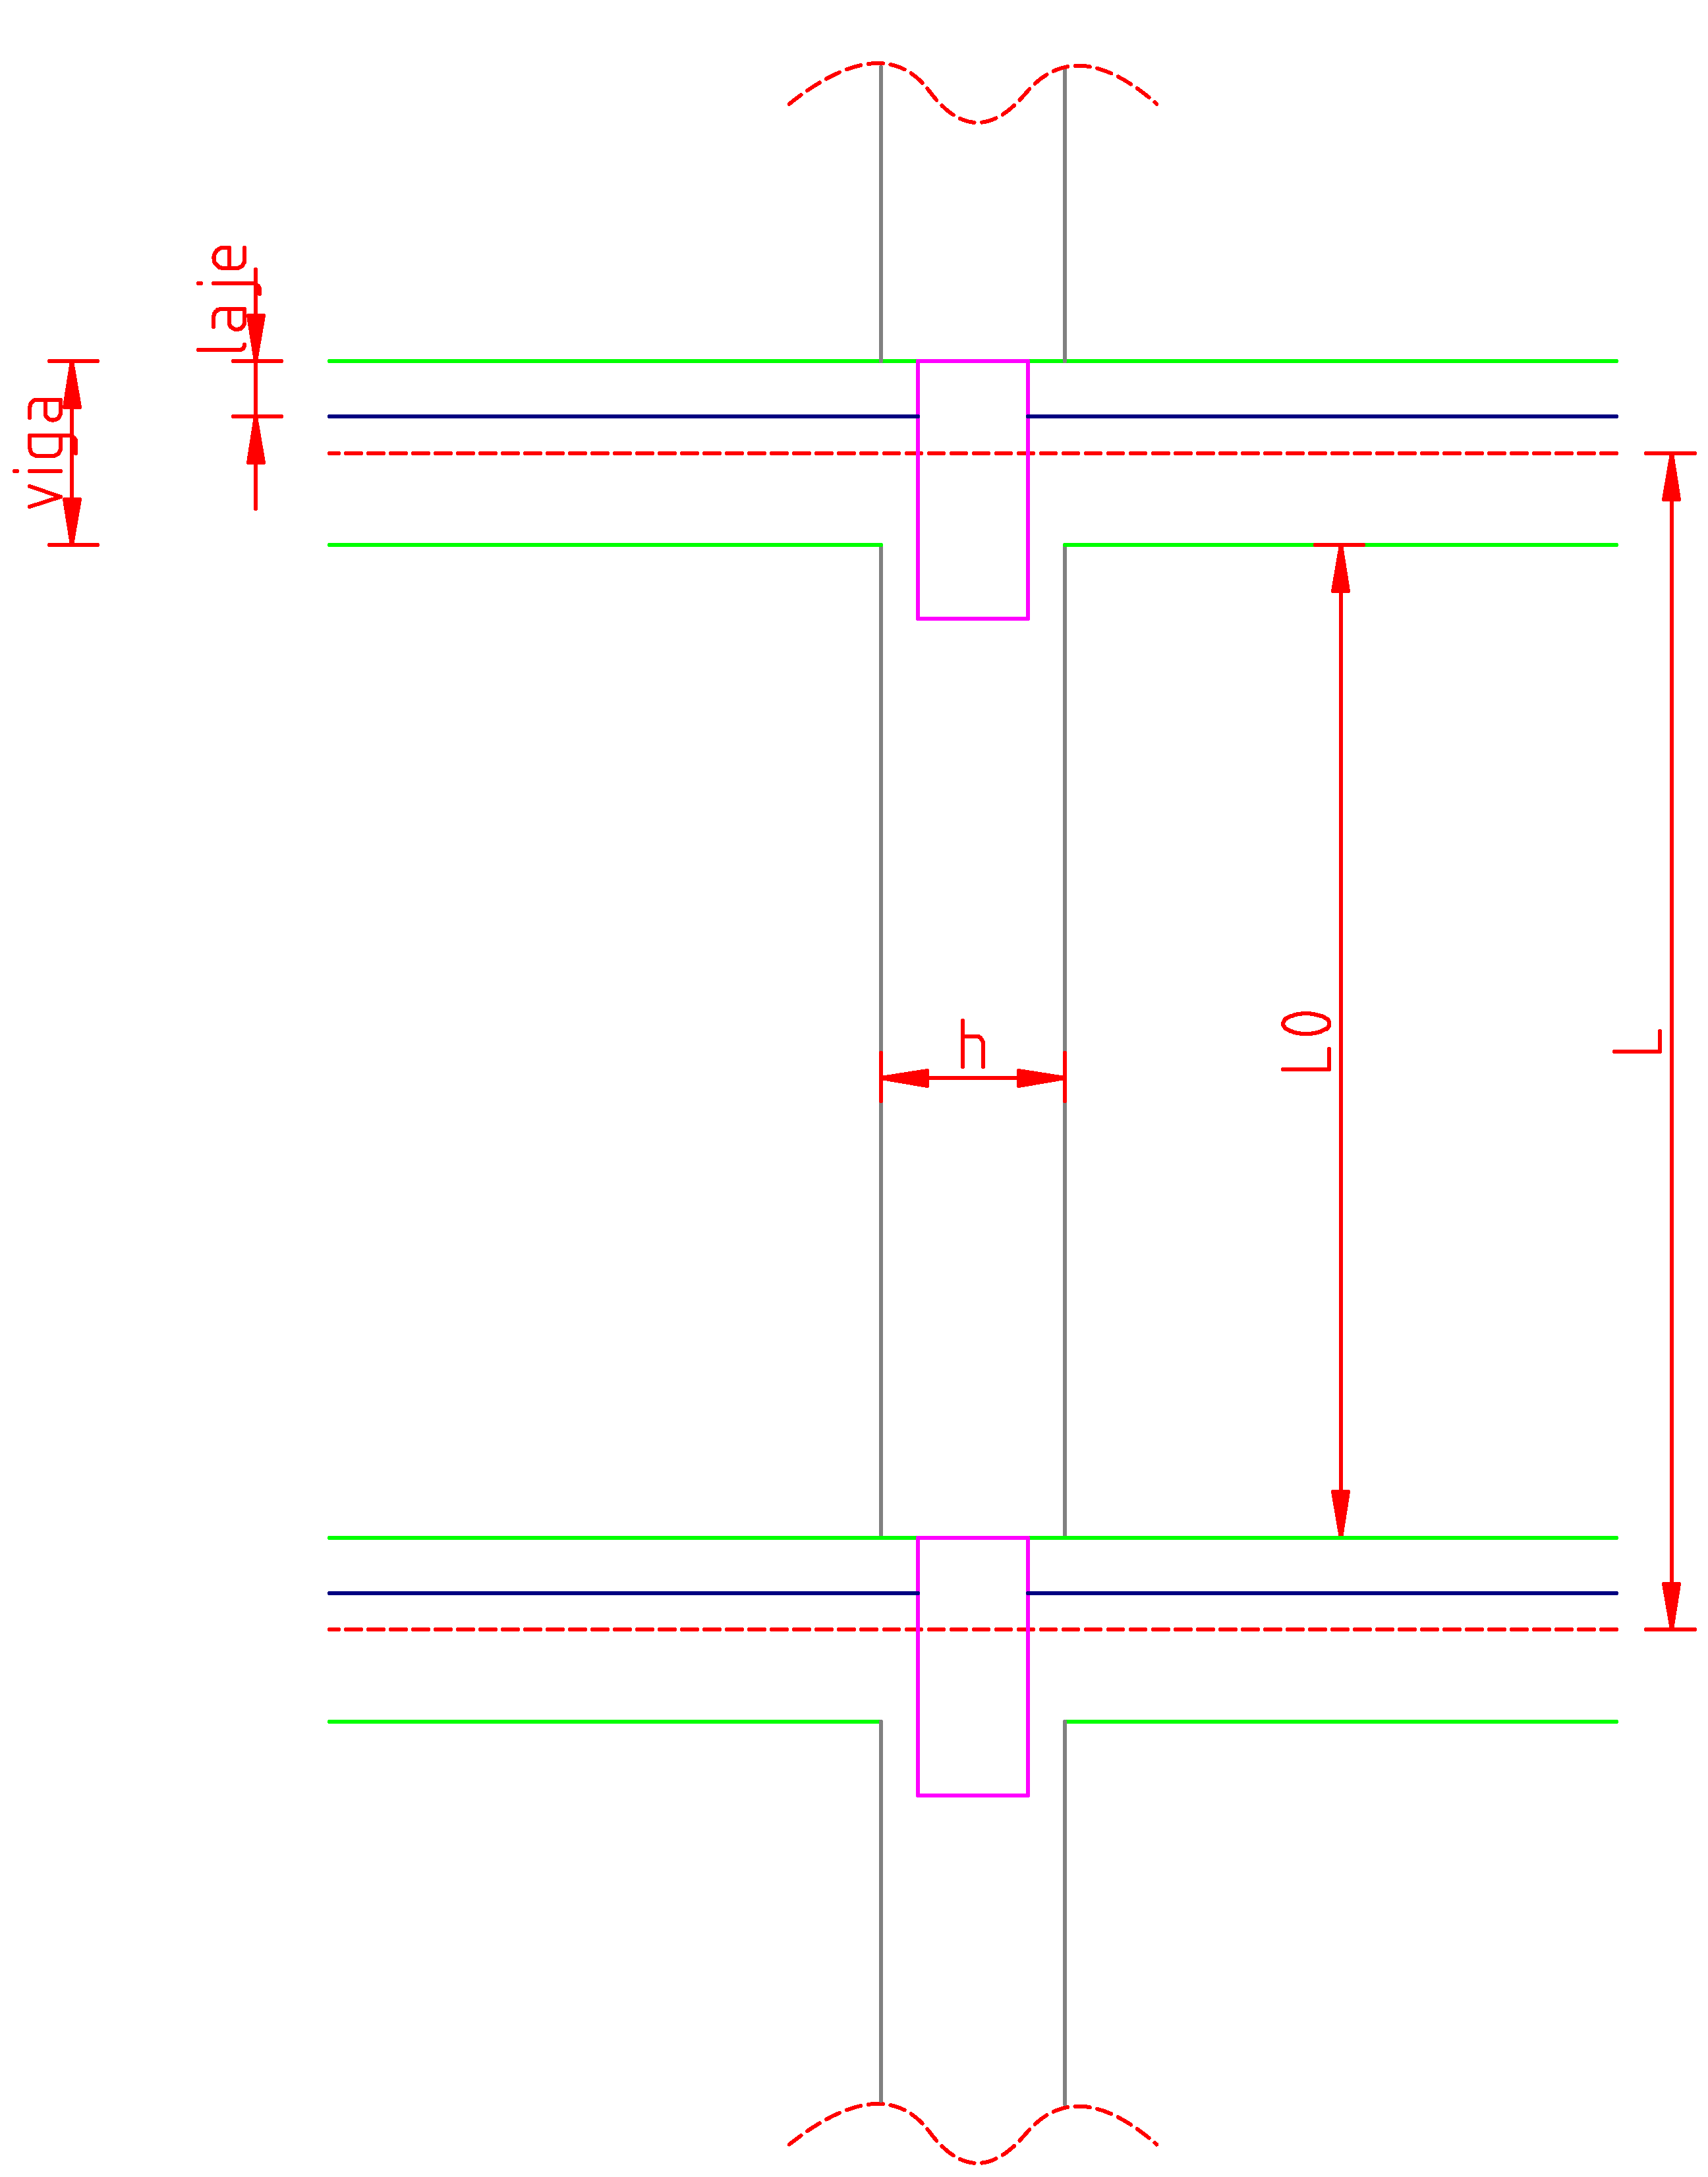
\includegraphics[width=0.7\textwidth]{Comprimento-equivalente/Imagens/Comprimento-equivalente.png}
	\end{center}
\end{figure}

\begin{equation}
	\label{equacao-comprimento-equivalente}
	L_e\leqslant\left\{
		\begin{array}{ll}
		L_0+h \\
		L
		\end{array}\right.
\end{equation}

Onde $L_0$ é a distância entre faces internas dos elementos estruturais, supostos horizontais, que vinculam o pilar, ou seja, a distância do topo da viga inferior à base da viga superior; $h$ é a dimensão da seção transversal do pilar, medida no plano da estrutura em estudo (eixo $x$ e $y$); e $L$ é a distância entre os eixos dos elementos estruturais aos quais o pilar está vinculado (distância do eixo da viga inferior ao eixo da viga superior).

Exercício: Definir o comprimento equivalente do pilar abaixo para as direções $x$ e $y$, considerando a seguinte figura para um pilar P1(35x60):

\begin{figure}[H]
	\begin{center}
	\caption{Configuração de um pilar genérico P1 .}
    	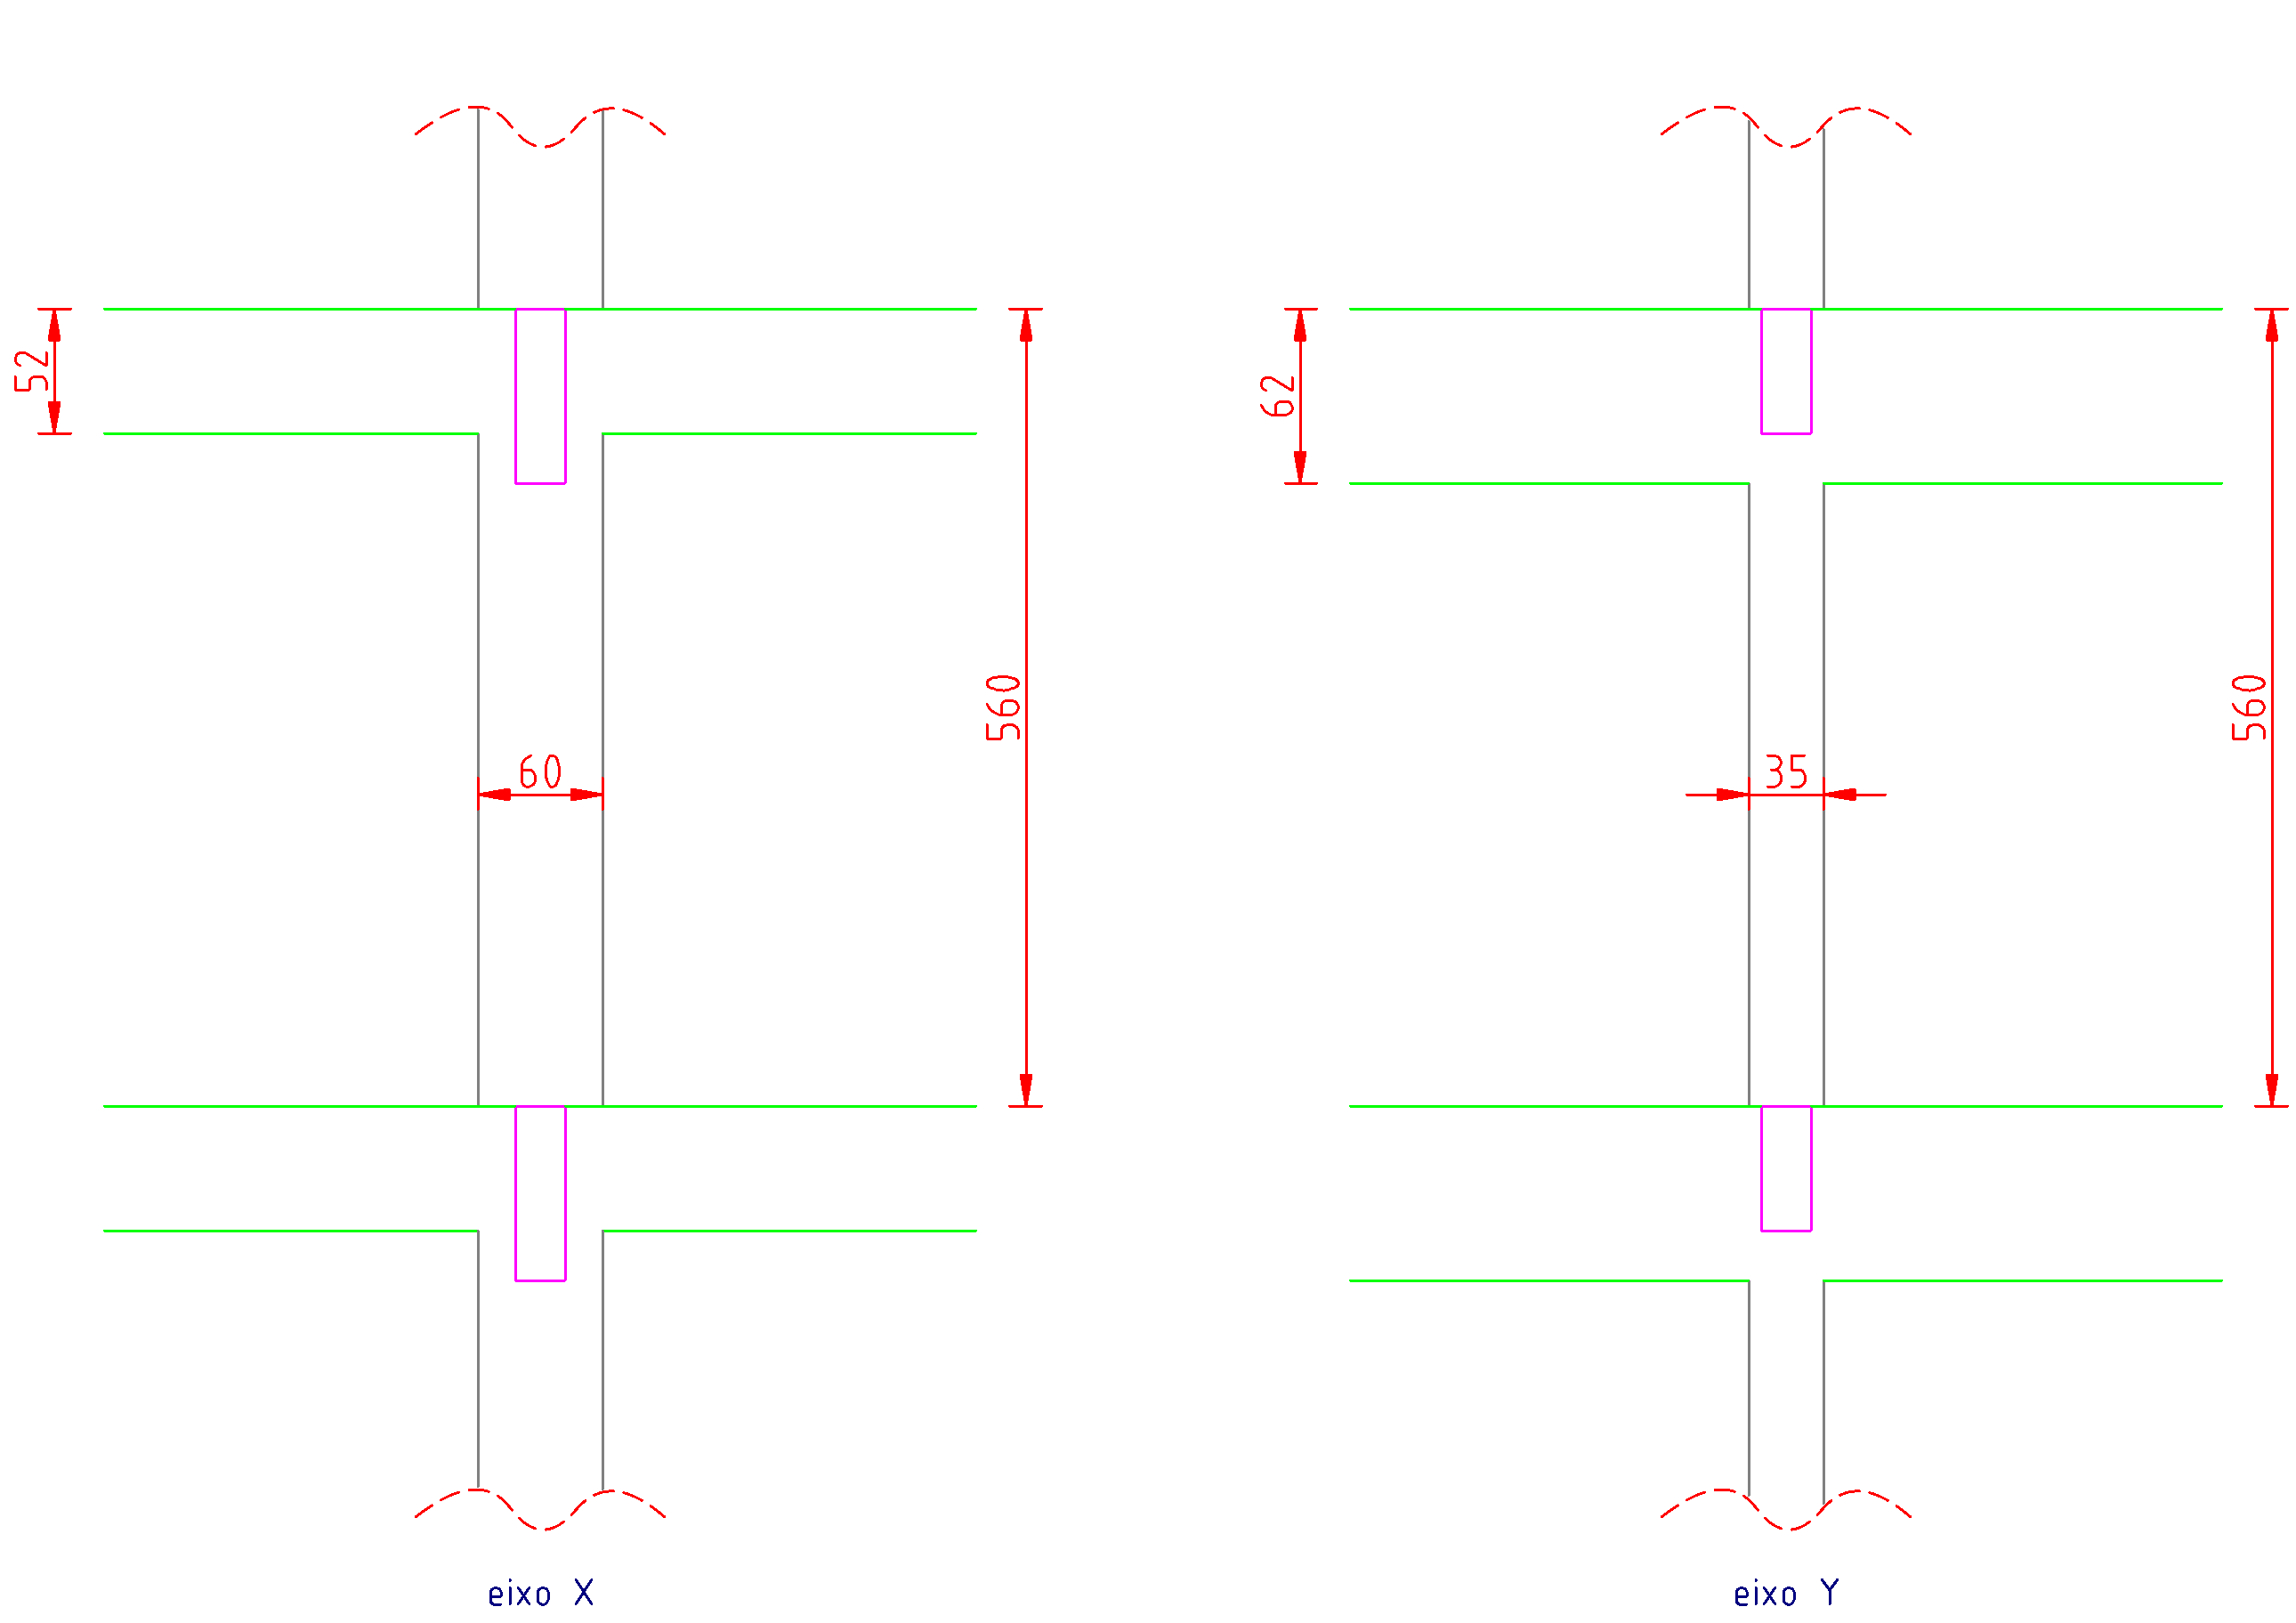
\includegraphics[width=0.85\textwidth]{Comprimento-equivalente/Imagens/Comprimento-equivalente-exercicio.png}
	\end{center}
\end{figure}
$$
	L_{e,\;x}\leqslant\left\{
		\begin{array}{ll}
		L_0+h=(560-52)+60=568\;cm \\
		L=\textbf{560\;cm}
		\end{array}\right.
$$
$$
	L_{e,\;y}\leqslant\left\{
		\begin{array}{ll}
		L_0+h=(560-62)+35=\textbf{533\;cm} \\
		L=560\;cm
		\end{array}\right.
$$



	\section{Comprimento de flambagem}
	A deflexão lateral produzida por uma carga sobre um pilar compõe o processo conhecido como \textbf{flambagem por flexão}. Ela ocorrerá sempre em torno do eixo de menor momento de inércia de sua seção transversal, pois gerará o maior índice de esbeltez.

Para calcular o índice de esbeltez é necessário o comprimento de flambagem, que é dado de acordo com o tipo de vinculação na base e no topo do pilar.

*Inserir figura

Porém, a NBR 6118, item 15.8.2 diz: Caso seja pilar engastado e livre no topo, o valor de $L_e=2\cdot L$. Nos demais casos, adotar os valores calculados anteriormente pela Equação~\eqref{equacao-comprimento-equivalente}.


	\section{Índice de esbeltez}
	\input{Indice-de-esbeltez/Índice-de-esbeltez.tex}

\end{document}